\documentclass[12 pt]{article}
\usepackage{hyperref}
\usepackage{fancyhdr}
\usepackage{setspace}
\usepackage{enumerate}
\usepackage{amsmath}
\usepackage{lastpage}
\usepackage{mathtools,float}
\usepackage{tikz}
\usepackage{listings}
\usepackage[margin=1 in]{geometry}
\allowdisplaybreaks
%\usepackage[dvipsnames]{xcolor}   %May be necessary if you want to color links
\hypersetup{
	%colorlinks=true, %set true if you want colored links
	linktoc=all,     %set to all if you want both sections and subsections linked
	linkcolor=black,  %choose some color if you want links to stand out
}
\usepackage{graphicx}
\graphicspath{{Images/}}
\author{Julian Lore}
\date{Last updated: \today}
\title{COMP 273: Intro to Computer Systems Review}
\pagestyle{fancy}
\lhead{COMP 273}
\chead{\leftmark}
\rhead{Julian Lore}
\cfoot{Page \thepage \ of \pageref{LastPage}}
\newcommand{\tab}[1]{\hspace{.2\textwidth}\rlap{#1}}
\begin{document}
	\onehalfspacing
	\maketitle
	Adapted from Joseph Vybihal's Winter 2017 COMP273 slides.
	\\ Some things taken from \href{https://www.allanwang.ca/}{Allan Wang's website}.
	\tableofcontents
	\newpage
	\section{Basics}
	\subsection{Bytes}
	A \textbf{byte} consists of 8 bits, 8 inputs and outputs. The main thing we will be working with in this course.
	\\ 5v signifies T/1, whereas 2v signifies F/0.
	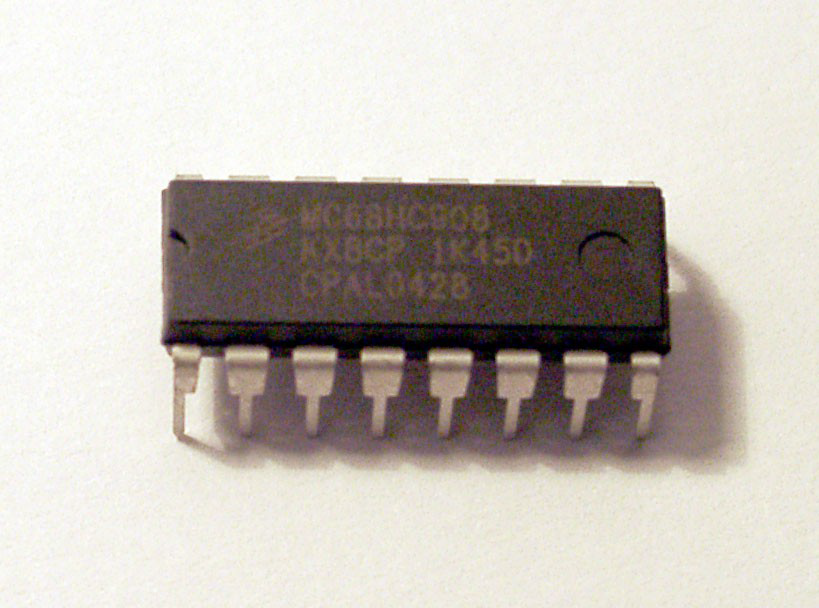
\includegraphics[scale=0.1]{byte.png}
	\\ Bytes consist solely of 3 gates (AND, OR, NOT), other gates can be made from these. 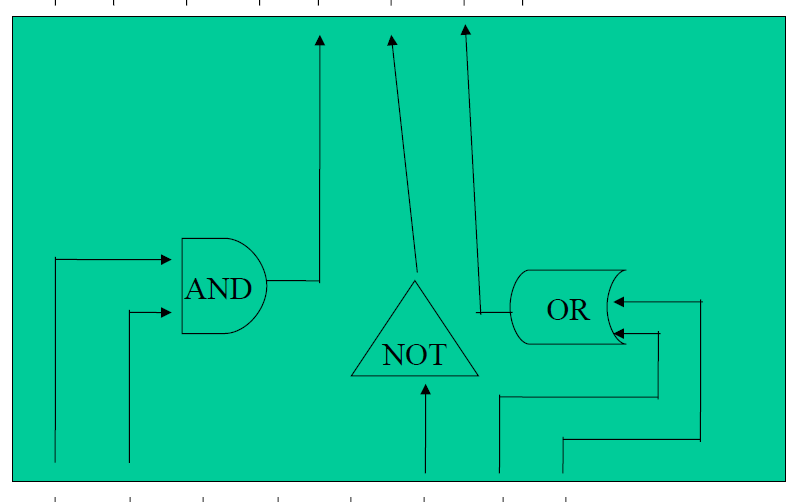
\includegraphics[scale=0.3]{gates.png}
	\subsection{Electricity Flow}
	Electricity flows like water on a flat surface, will go in all directions. In order to control electricity flow, we will use \textbf{gates}.
	\\ If electricity flows the opposite way it's supposed to (in where it's out), the computer will freeze.
	\section{System Board}
	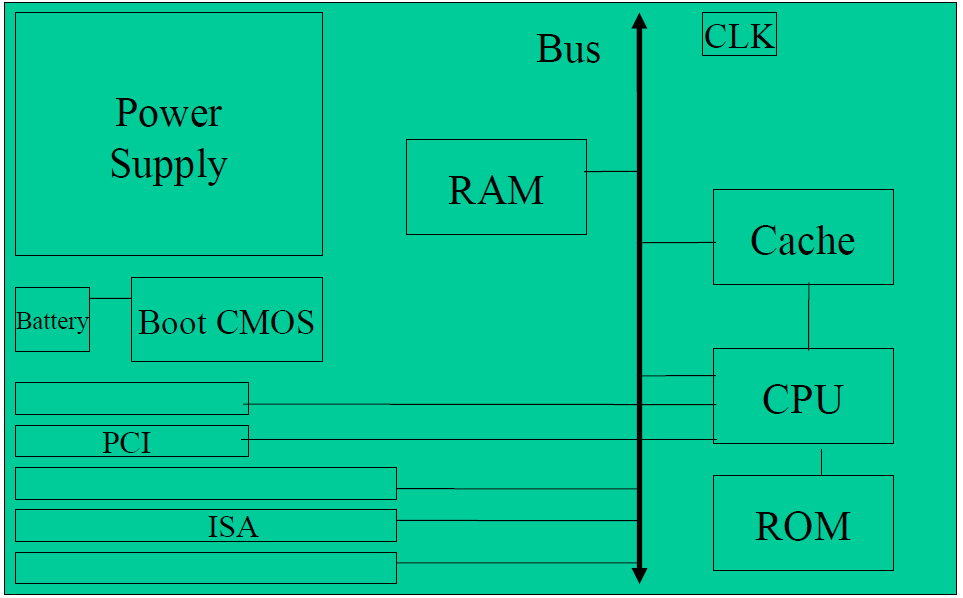
\includegraphics[scale=0.5]{sb.png}
	The system board consists of data paths, such that everything is connected.
	%
	\\ Many definitions on Lecture 1, are they needed?
	%
	\subsection{Bus}
	The \textbf{bus} links everything together on the system board. A conduit for bytes to travel from one location to another location (pathway). On the classical CPUs, there is only 1 bus, so only 1 thing can use the bus at once.
	\\ 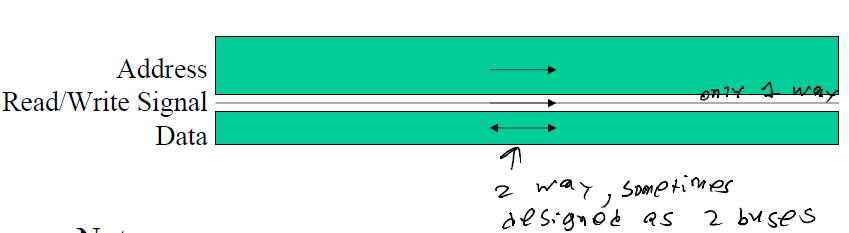
\includegraphics[scale=0.6]{bus}
	\\ Here's an optimized schematic that uses the bus less. It provides several direct/private data lines:
	\begin{itemize}
		\item From the CPU to the cache (cache can operate at CPU clock speed)
		\item Cache to RAM
		\item CPU to PCI
		\item All of these make things faster
		\item Great use of speediness of CPU
	\end{itemize} %from the CPU to the cache (for lots of speed) and a line from 
	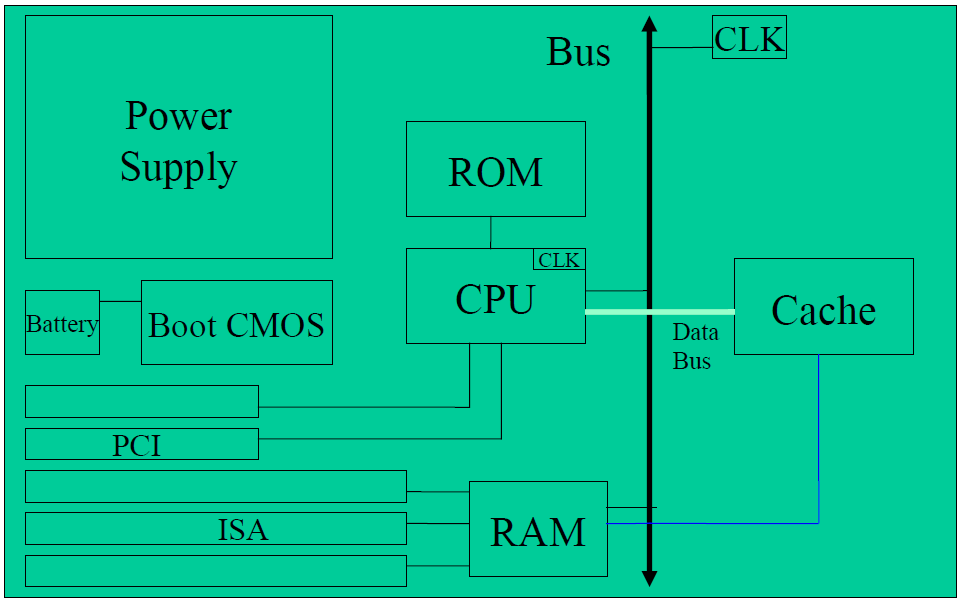
\includegraphics[scale=0.5]{sbo.png}
	\\ Can multi-thread with multiple buses, but multiplies the cost of the computer
	\subsection{Pathways}
	There are many other \textbf{pathways}, such as system buses (ISA, PCI), data bus, CPU bus, wires. These pathways are to \textbf{interconnect} components. Pathways are composed of multiple parallel wires (to be executed independently), one wire per bit. One byte goes through a bus per tick. 
	\paragraph{Shorthand for multiple wires}8 wires
	\begin{tikzpicture}[scale=0.3]
		\draw (0,0)--(5,0);
		\node (8) at (4,2){8};
		\draw (2,-1)--(8);
	\end{tikzpicture}
	\subsection{RAM}
	Volatile (live data) general purpose main memory bank, large \& slow, \textbf{RAM} consists of addresses, storage space and the zero page, which connects to slots. Comparable to an array.
	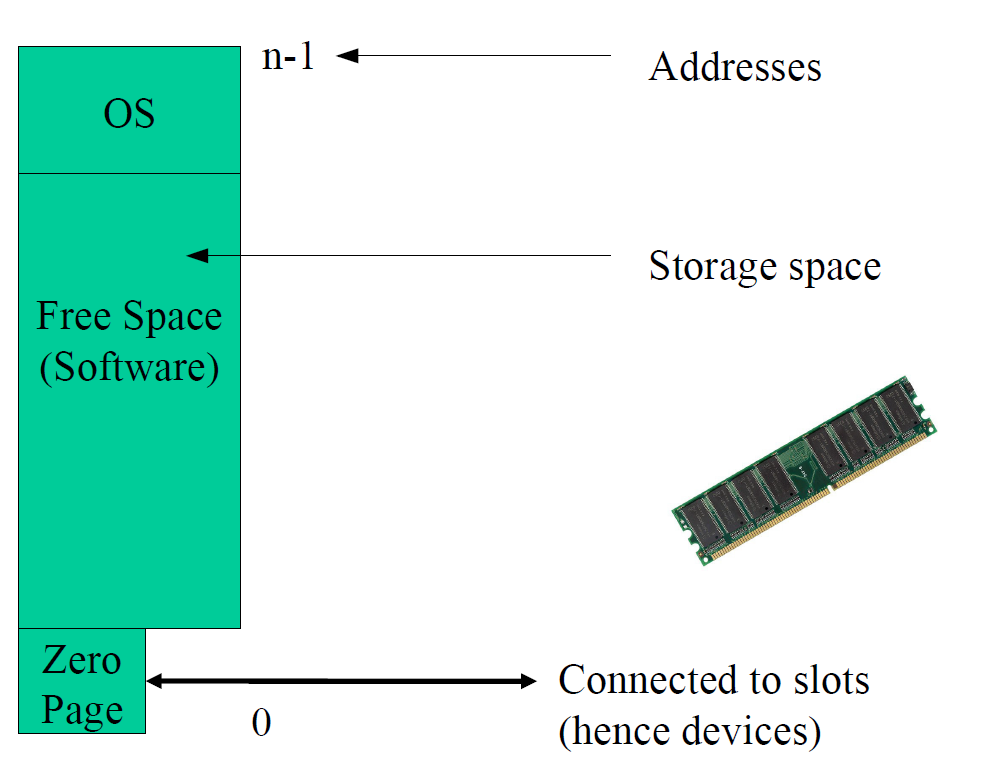
\includegraphics[scale=0.3]{rm.png}
	In comparison to cache, RAM costs pennies and cache costs dollars. Cache is much faster, but RAM is used as an illusion to make the computer work as if all the memory was cache.
	\\ RAM separated into 2 sections, addresses and data. RAM is actually mostly addresses. \textbf{Data} is typically 8 bits, whereas the size of addresses varies. Typically 32 or 64 bit right now, soon to be 128. Once RAM is built with some size, you can't change it (so you must decide wisely). Need 1 wire per bit (i.e. 8 wires going to data part and however many for addresses). In order to r/w to RAM, we need a few things. \textbf{Address register} to select address/row, mode register for r/w and data register. For large values/things, like strings, store in consecutive memory areas.
	\paragraph{Video and RAM}
	1:1 correspondence with RAM and pixels. Pixels represented by integer numbers. 
	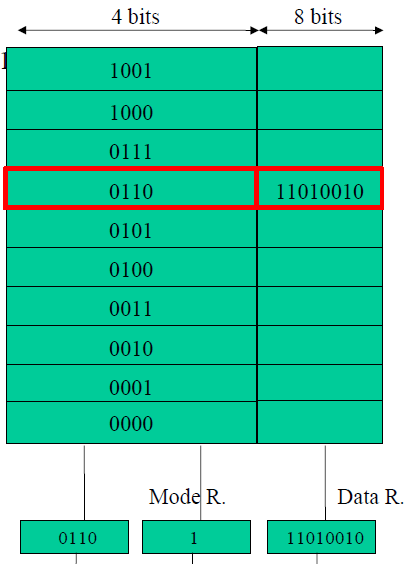
\includegraphics[scale=0.3]{rrr.png}
	\subsection{Clock}
	There are always at least 2 \textbf{clocks}. One for the bus (much slower) and one for the CPU (much faster). The bus clock is 1 or 2 orders of magnitude slower than the CPU clock.
	\paragraph{Bus Clock}
	\begin{itemize}
		\item Mainly for gating access to bus.
		\item Also regulates data movement on system board.
	\end{itemize}
	\paragraph{CPU Clock}
	\begin{itemize}
		\item Responsible for instruction execution inside CPU.
		\item Moves data using CPU bus or moves code from IP $\to$ sequencer
		\item Doesn't affect things outside CPU.
		\item The clock will determine order of instruction execution (they have to take turns).
	\end{itemize}
	\subsection{PCI \& ISA}
	Connect outside of the computer, to other peripherals like monitors. PCI can run at higher clock speeds than ISA.
	\subsection{Addressing}
	All components of system board have a unique integer number identifying them. Needed, so that we can block electricity from going to certain peripherals.
	\subsection{CPU}
	Central Processing Unit, used for math, logic, data, movement \& loops.
	The \textbf{CPU} is pretty simple/basic, even though it's the ``brain" of the computer. It's main capabilities consist of adding, subtracting, multiplying, knows about the 3 gates.
	\paragraph{Classical CPU Scheme Without Cache} ~
	\\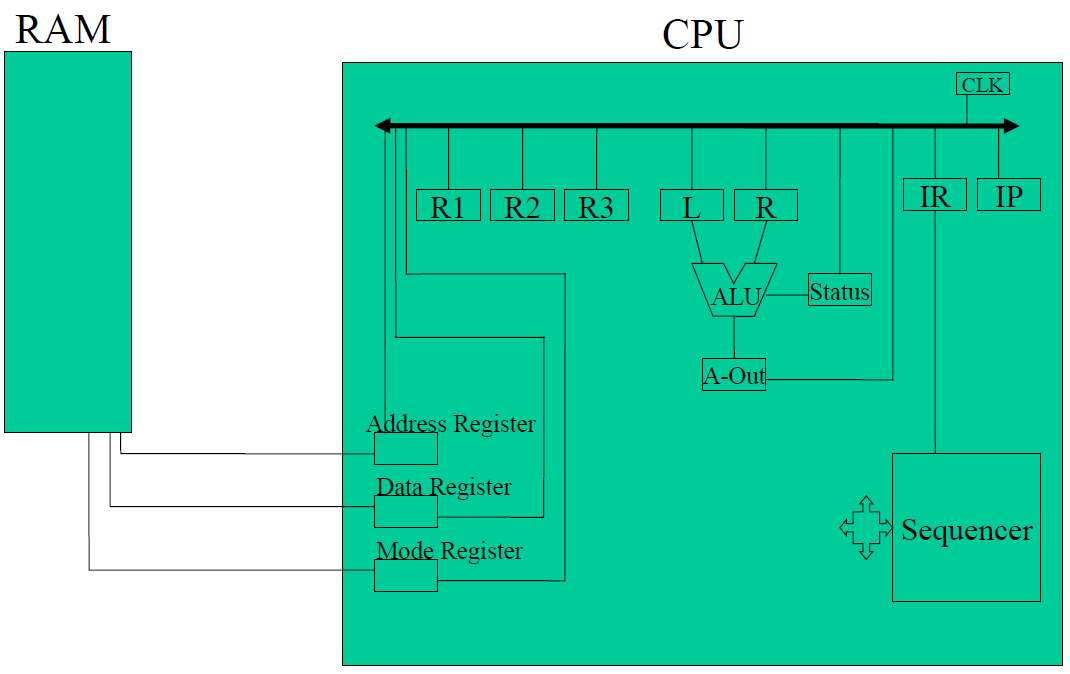
\includegraphics[scale=0.5]{cpu.png}
	Here, RAM reads the address from the address register, writes to the data register and the mode register differentiates read/write. The sequencer opens and closes gates.
	\paragraph{Registers}
	Like temp variables for the CPU. Store single value.
	\paragraph{ALU: Arithmetic Logic Unit}
	The ALU takes 2 inputs, L and R to get it's output, A-Out. The Status register takes input (for type of operation) and output to report errors, like overflow, dividing by zero.
	\\ ALU consists of a bunch of adders, 2s complement circuit for L and for R (need something that inverts bits and then use an adder to increment by 1).
	\paragraph{IP(Instruction Pointer) or IC (Instruction Counter)}
	\begin{itemize}
		\item Next instruction/address to execute
		\item Address Register points to it when needed
	\end{itemize}
	\paragraph{IR (Instruction Register)}
	\begin{itemize}
		\item Current instruction being executed
		\item From data register
		\item First part is op-code, goes to control unit
		\item Parts after are arguments
		\item Usually 3 args, $3^{rd}$ is usually optional?
	\end{itemize}
	\subparagraph{Example Instructions}
	\begin{itemize}
		\item lw \$2, (\$3) (indirect)
		\begin{itemize}
			\item Loads word into reg 2 from address in reg 3
		\end{itemize}
		\item lw \$2, \#1A2F
		\begin{itemize}
			\item Goes directly to address, no need to check register (direct)
		\end{itemize}
		\end{itemize}
	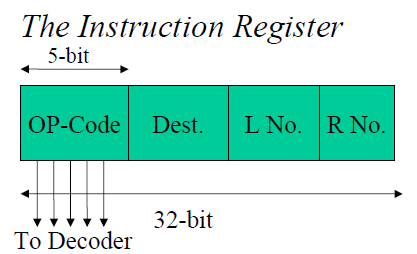
\includegraphics[scale=0.5]{ir.png}
	\begin{itemize}
		\item L $\to$ L register
		\item R $\to$ R register
		\item A-Out $\to$ Dest
		\item OP-Code is used by sequencer to trigger circuit that will do this action.
	\end{itemize}
	We can't distinguish variables, addresses and operations.
	\paragraph{RAM Access Register System}
	\begin{itemize}
		\item Communicates CPU $\leftrightarrow$ RAM
		\item Address register (r/w this address)
		\item Data register (data received or sending)
		\item Mode register (r/w)
	\end{itemize}
	\paragraph{CPU Boundary Register} Keeps track of addresses used, addresses requested shouldn't pass boundary address.
	\paragraph{Sequencer/Decoder}
	\begin{itemize}
		\item Table, codes with circuits
		\item Circuits have gated triggers, allowing data to go in a specific order
		\item Sequencer and ROM have circuitry to react to machine lang, allow computer to execute instr. Sequencer: built-in instr. ROM: extended instr.
	\end{itemize}
	\paragraph{CPU Clock}
	See 2.4.
	\paragraph{CPU Loop (Execution)}
	\begin{enumerate}
		\item Get instruction: IR $\gets$ RAM (or cache), slow bus
		\item Sequencer $\gets$ IR[op-code]
		\item Selected gates open
		\item Clock ticks (if this is outside CPU, have to respect other clocks too)
		\item All gates close
		\item Increment  $\to$ next instruction (fast). Back to step 1.
	\end{enumerate}
	Shorthand: 
	\begin{enumerate}
		\item AR $\gets$ PC
		\item PC $\gets$ PC+1
		\item DR $\gets$ RAM[AR]
		\item IR $\gets$ DR
		\item Re-loop
	\end{enumerate}
	Constant switch from slow to fast clock means we are never really fast, which is why we need things like a cache.
	\paragraph{Memory}
	Different types of memory. See specific sections for more info.
	\begin{itemize}
		\item RAM (primary storage). DRAM: Dynamic, must refresh. SRAM: Static, no refresh.
		\item ROM, read only memory (advanced instructions). ROM is hardwired. PROM programmable once (fuses). EPROM, erasable by heat. EEPROM electrically erasable. PAL, PLA.
		\item Cache. Very fast memory, usually on CPU. Store frequently accessed info. Doesn't use system bus. 1 direction, cache1 $\to$ CPU and CPU $\to$ cache2.
		\item Pipeline. Use assembly line to process instructions. Partially parallel. Series of instruction registers.
	\end{itemize}
	\section{Data/Data Encoding}
	\textbf{Data} is information stored in RAM or secondary storage. Can be instructions or information. There are built-in types CPU can understand (int, real, char), since there are circuits made to interpret them. Language types must be simulated. The \textbf{bit} is the fundamental unit of the computer. Using bits and gates, we will group things in order to store data.
	\paragraph{Bit Grouping}
	Two forms: numerical binary representation and tabulated binary encoding (ASCII, UNICODE, instructions, etc.). Can count, add, subtract, multiply and divide with binary numbers. 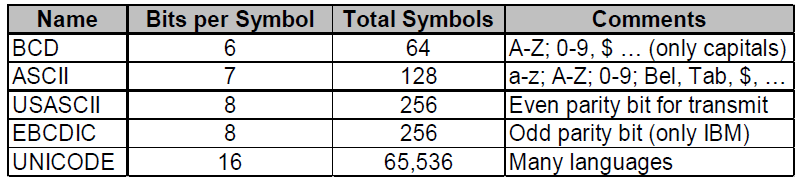
\includegraphics[scale=0.4]{asc.png} 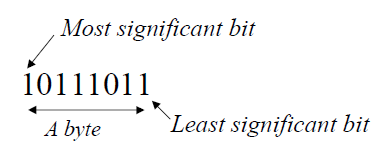
\includegraphics[scale=0.5]{bsg}\\
	How to represent data? How many bits do we need? What medium to use? (lights, sound, signals) Lightbulbs originally used, either on or off. \begin{tabular}{|c|c|}
		\hline Nibble & 4 bits \\ \hline Byte & 8 bits \\ \hline Word & 16 bits \\ \hline Long Word/Word & 32 bits \\ \hline Quad Word/Word & 64 bits \\ \hline
	\end{tabular} There are standards for data types/storage established by IEEE and ISO. 3 basic things to encode: chars, numbers and instructions. For \textbf{characters}, we use a predetermined table (ASCII, unicode), \textbf{numbers} use binary arithmetic and \textbf{instructions} use a table, gate sequence code-number.
	\paragraph{Word}
	Word is the common size of a register of CPU(best for design of CPU). CPUs often have multiple register sizes. Word sizes differ between CPUs. Nowadays, register size is usually the same as address size.
	\subsection{Data Types \& Encoding}
	How does the machine know that a byte is a character? The ROM (Read Only Memory), has predefined instructions to deal with it. Compiler will look at ASCII table and display the respective character, etc. 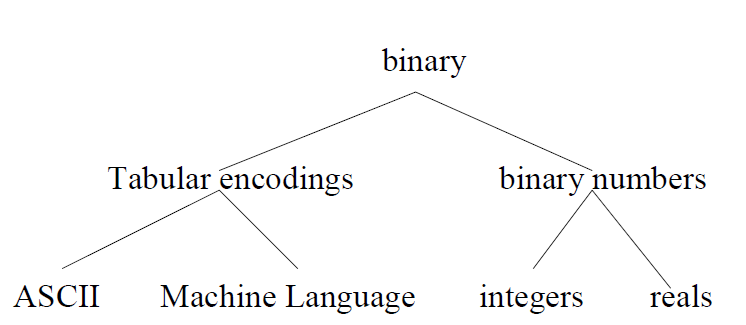
\includegraphics[scale=0.3]{btree} You need the ROM for tabular encodings, but not for binary numbers.
	\subsubsection{Number Representations}
	\paragraph{Binary} 
	\begin{itemize}
		\item Used for flags, numbers, strings, encodings
		\item Longhand addition in binary is the same as elementary grade addition with decimals
		\begin{itemize}
			\item But we have a fixed size
			\item If we carry past size $\to$ \textbf{Arithmetic Overflow}
			\item Signed overflow expected for 2's complement subtraction
		\end{itemize}
	\end{itemize}
	\paragraph{Hexadecimal} Easier to read for humans, better correspondence with binary. Base 16, with 10-15 being A, B, C, D, E, F. Decimal to Binary conversion is slow. Computers often convert binary to hex for errors to make it easier to read.
	\paragraph{Octal}
	\begin{itemize}
		\item Barely used anymore
		\item Except for Unix permissions and C, Perl escape codes
	\end{itemize}
	\subsubsection{Conversion}
	\paragraph{Decimal $\to$ Binary} Keep dividing by 2 until you get 0, read the remainders from bottom to top $\to$ left to right. 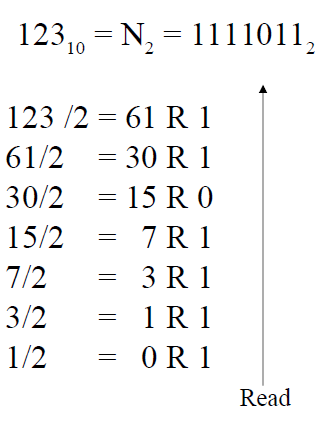
\includegraphics[scale=0.5]{dbc}
	\paragraph{Decimal $\to$ Hex} Divide by 16 until 0, read remainders in same way.\\ 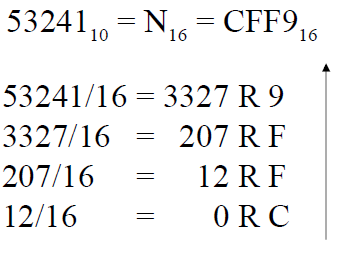
\includegraphics[scale=0.5]{dhc}
	\paragraph{Binary $\to$ Decimal} Depending on position of number, multiply value by $2^{\text{n}^{th} \text{position}}$
	\begin{equation*}
	1011_2=N_{10}=11_{10}=1\times 2^3 + 0 \times 2^2 + 1 \times 2^1 + 1 \times 2^0
	\end{equation*}
	\paragraph{Hex $\to$ Decimal} Same principle with base 16. 
	\begin{equation*}
	1AB_{16}=N_{10}=427_{10}=1\times 16^2 + A \times 16^1 + B \times 16^0
	\end{equation*}
	\paragraph{Binary $\leftrightarrow$ Hex} 1 nibble = 1 hex digit
	\begin{equation*}
	\underbracket{1111}_{F}\underbracket{0011}_{3}\underbracket{0001}_{1}{\underbracket{0000}_{0}}=F310_{16}
	\end{equation*}
	\paragraph{Binary $\leftrightarrow$ Octal} 3 bits = 1 octal, same as Hex strategy.
	\subsubsection{Binary Encodings}
	\paragraph{ASCII} $2^7$ values, but wasn't enough for special characters like accents.\\ 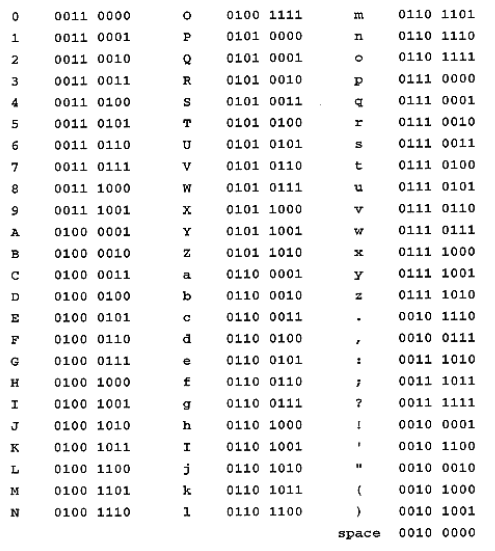
\includegraphics[scale=0.7]{basc}
	\subsubsection{Data Representation}
	Representing data consists of a choice, that comes at a cost. Pros/cons to each choice. Specify the base when writing numbers in this class. 3 representations:
	\begin{itemize}
		\item Logical description (how it truly looks \& behaves)
		\item Physical construction
		\item Circuit
	\end{itemize}
	We need legal operators, abstraction of what is being recorded (chars don't exist) and want to know how we want to represent information in binary (size, addressing).
	\paragraph{Integers} Usually 16,32 or 64 bits. How do we differentiate sign? We can have a \textbf{signed} bit (use most significant bit as sign) or use ``2's complement". With signed bits, there exists a negative 0, but with 2's comp, only one 0 and most significant bit is still a sign bit. We don't need a null at the end of an int, it's matched with x bit instructions made for its size. 
	\subparagraph{Two's Complement} Easier to build computers if they subtract using: 
	\begin{equation*}
		X-Y=X+(-Y)=X+(\text{2's complement of Y})
	\end{equation*}
	How to convert? \begin{itemize}
		\item Take Y
		\item Flip bits
		\item Add 1
		\end{itemize} 
		Uses a signed overflow in order to get expected result.
	\subparagraph{Example}
	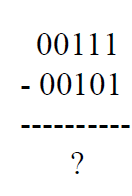
\includegraphics[scale=0.5]{22} 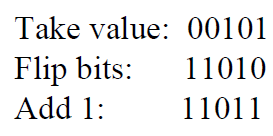
\includegraphics[scale=0.5]{22a} 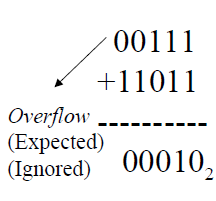
\includegraphics[scale=0.5]{22b}
	\subparagraph{Base 10 Two's Complement}
	\begin{align*}
		&-N = Base^{size}-N \\
		&-12_{10}=10^2-12=88_{10} \\
		&15-12=15+88=103 \implies \text{Drop carry, get }3
	\end{align*}
	\subparagraph{Signed vs 2's Comp}
	\begin{itemize}
		\item Signed \begin{itemize}
			\item Easy to read
			\item No conversion
		\end{itemize}
		\item 2's
		\begin{itemize}
			\item Unique 0
			\item Auto subtracts when adding
		\end{itemize} 
		\end{itemize}
	\paragraph{Characters} Encoded using ASCII or UNICODE or something similar (standard). Type not stored in computer, there are no types.
	\paragraph{Strings} Each char stored in 1 byte in RAM (consecutive). Either a null at the end signifying the end of the String, or the most significant bit describes length.
	\paragraph{Floating Point/Real Numbers} Scientific notation approximation, store decimal and exponent.
	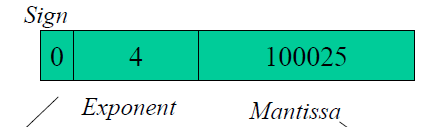
\includegraphics[scale=0.5]{fp} 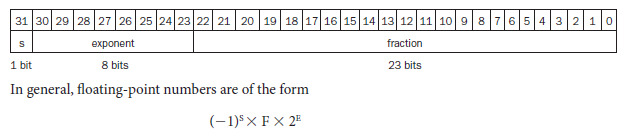
\includegraphics[scale=0.6]{fp32}
	\subparagraph{IEEE format} Uses bias for exponent, i.e. for 32 bit, 127=0, 126=-1, 128=1. This way we don't need a signed bit.
	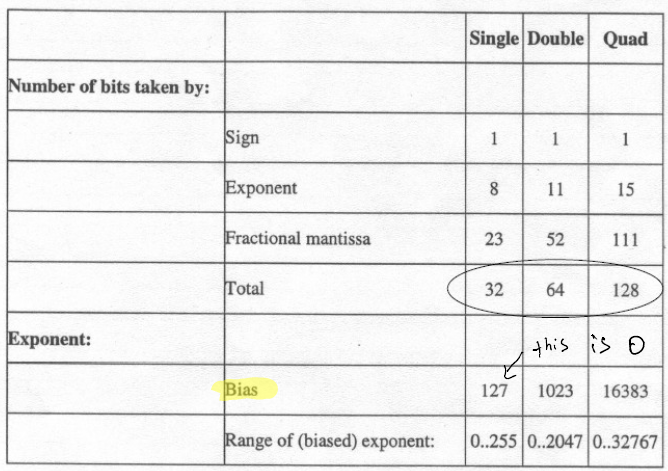
\includegraphics[scale=0.5]{ieeefp}
	\\ Mantissa stores a fraction(raw digits after decimal) for approximation. Normalize your fraction such that you get 1.something and ignore the 1. \subparagraph{Example}
	\begin{align*}
		& -0.75_{10}=-3/4_{10}=-3/2^2_{10} \\
		& \implies -11_2/2^2_{10}=-0.11_2=-0.11_2 \times 2^0=-1.1_2 \times 2^{-1}
		\\& \implies (-1)^1 \times (\underbrace{1}_{ignored}+ .100 \ldots 00_2) \times 2^{126-217}
	\end{align*}
	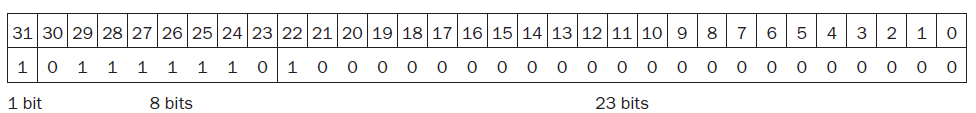
\includegraphics[scale=0.7]{exfpm}
	Notice that the leading 1 before the decimal is ignored. The $22^{nd}$ bit is $2^{-1}$, the $23^{rd}$ is $2^{-2}$, etc. Since we had $1.1_2$, we look at the numbers after the decimal and just copy those.
	\paragraph{Logical}
	Single bit, 0=false, 1=true
	\paragraph{Packed Decimal}
	One nibble per digit of a number in base 10. Can be used to store decimal numbers. Addition is strange. Add 2 nibbles together, if you get over 10, subtract 10 and carry and add 1 over to next nibble. (i.e, if you do 3+9, you'll get 12 (5 bits), subtract 10 and represent 2 in binary)
	\begin{equation*}
		5372_{10}=0101 \: 0011 \: 0111 \: 0010
	\end{equation*}
	Very user friendly, but wastes space and complicates hardware.
	\subsection{Mathematical Operation Algorithms for Floating Points}
	\paragraph{Addition}
	\begin{itemize}
		\item Normalize (floating point)
		\item Round if required
		\item Put numbers to same exponent (shift smaller to right until it's the same as larger)
		\item Add significands
		\item Normalize (check for over/underflow)
		\item Round
		\item Sign?
		\end{itemize}
	\subparagraph{Ex} Add $0.5_{10}$ and $-0.4375_{10}$
	\\
	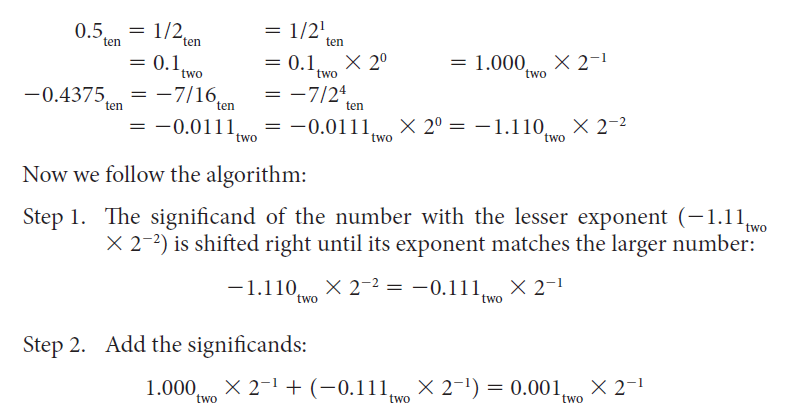
\includegraphics[scale=0.8]{exfa}\\
	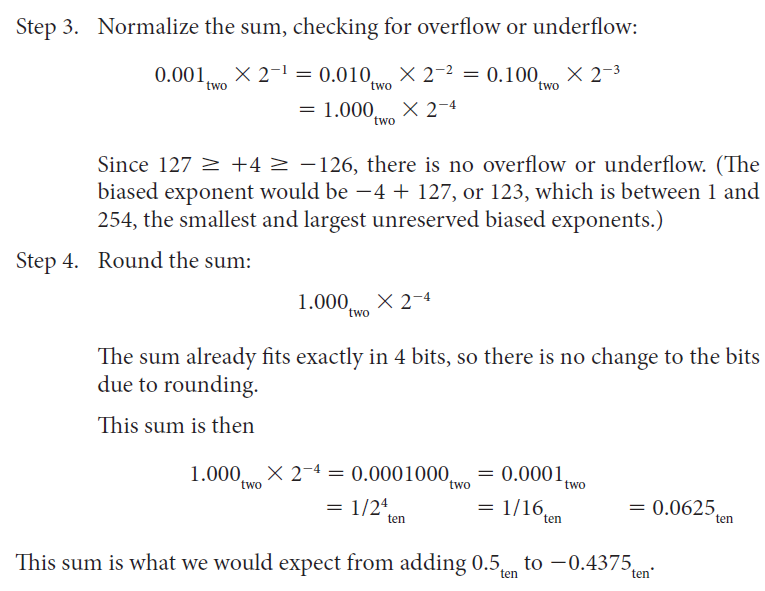
\includegraphics[scale=0.8]{exfaa}
	\paragraph{Multiplication}
	\begin{itemize}
		\item Remove exponent bias
		\item Match exp
		\item Multiply significands
		\item Normalize \& round
		\item Sign
	\end{itemize}
	\paragraph{Ex} Multiply $0.5_{10}$ and $-0.4375_{10}$\\
	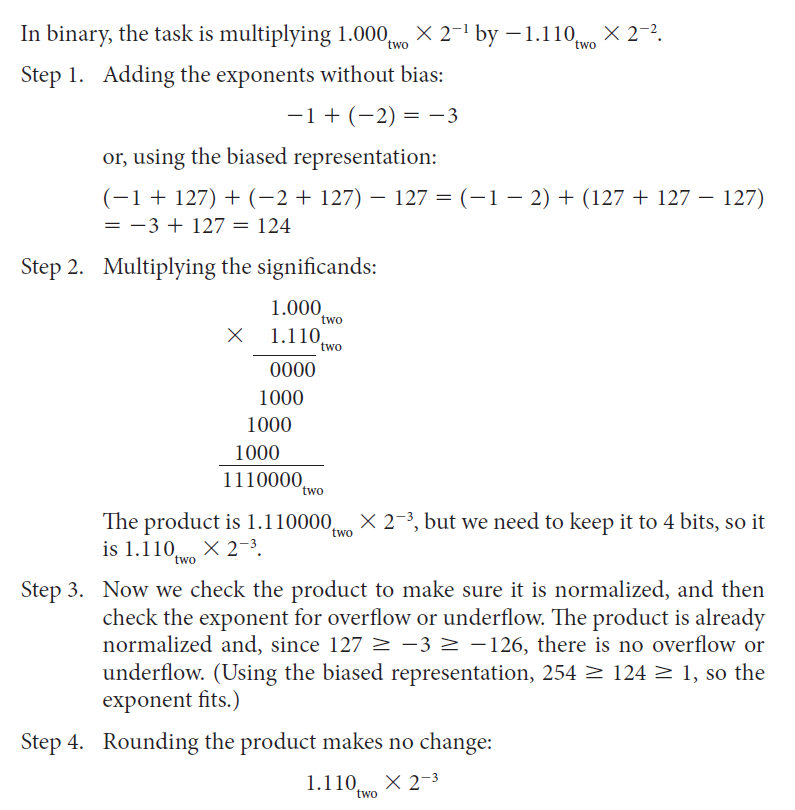
\includegraphics[scale=0.8]{fpm}
	\\ 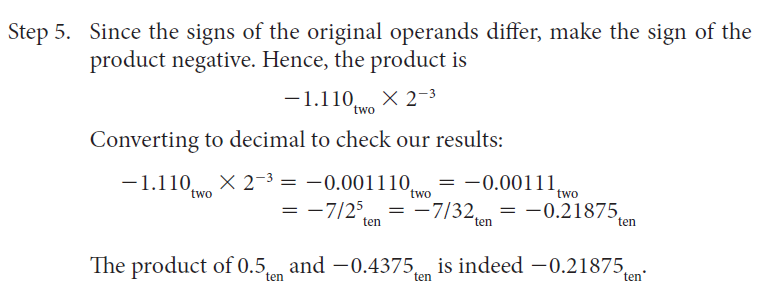
\includegraphics[scale=0.8]{fpma}
	\section{Logic \& Gates}
	\begin{itemize}
		\item 
		Circle $\implies$ not
		\item Extra line $\implies$ exclusive
	\end{itemize}
	\begin{figure}[H]
		\caption{Taken from \href{https://www.allanwang.ca/notes/mcgill/comp273/0.php}{Allan Wang's website}}
		\begin{center}
			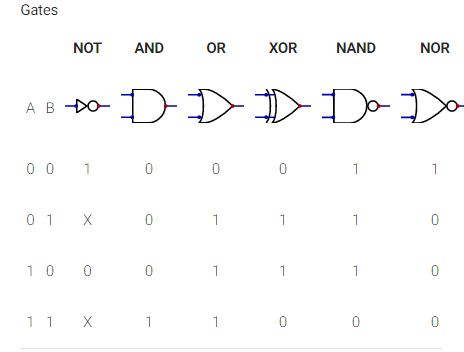
\includegraphics{gatess}
		\end{center}
\end{figure}
		Wire crosses, i.e. when are two wires connected: 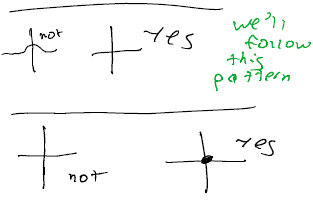
\includegraphics{wc}
		\paragraph{Low-level Construction}
		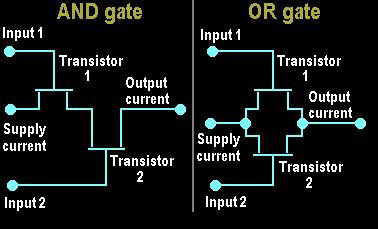
\includegraphics[scale=0.7]{aog}
		\\ 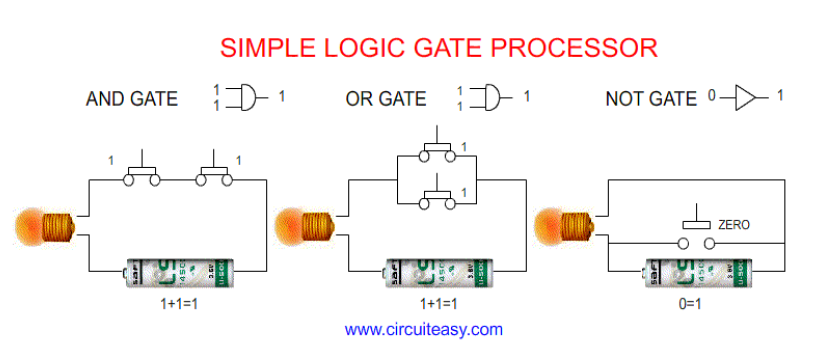
\includegraphics[scale=0.7]{lc}
	\subsection{Basic Flip Flop Circuits}
	\textbf{Flip Flops} are bits!
	\begin{figure}[H]
		\caption{RS Flip Flops, \href{https://www.allanwang.ca/notes/mcgill/comp273/0.php}{Allan Wang}}
		\begin{center}
			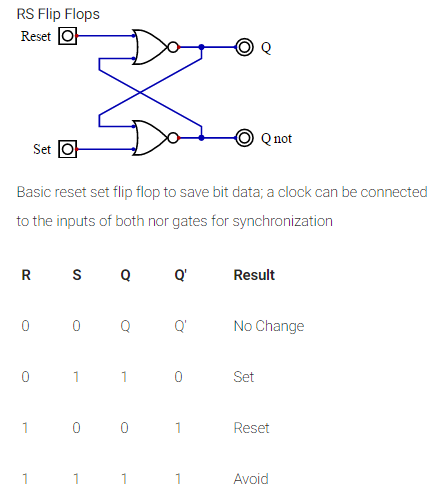
\includegraphics{rsf}
		\end{center}
		Sending 1 to reset(R) and set(S) is an invalid input. They must be opposites, or both 0. Sending a 1 through set, sets the bit's output, Q to 1, and it's complement Q' to 0. Sending 1 through reset does the opposite. If both are 0, keep current value (clocked).
		\\ Can test \textbf{steady state} of the circuit. Give a 1 to R and follow the circuit, realize nothing conflicts. The flip flops don't actually store anything, they just have data going through them $\to$ live data, lost when unplugged.
	\end{figure}
	Clocked RS: 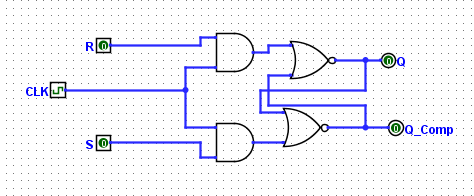
\includegraphics{clksr}
	Like an RS Flip-Flop, except only let's things through when clock ticks.
	\begin{figure}[H]
		\caption{JK Flip Flop, \href{https://www.allanwang.ca/notes/mcgill/comp273/0.php}{Allan Wang}}
		\begin{center}
			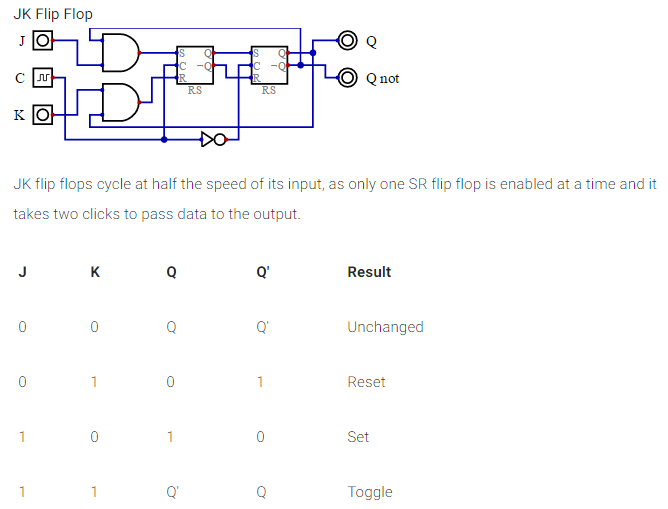
\includegraphics{jkc}
		\end{center}
		2 SR flip flops, adds a delay.
	\end{figure}
	\begin{figure}[H]
		\caption{D Flip Flop/D Latch, \href{https://www.allanwang.ca/notes/mcgill/comp273/0.php}{Allan Wang}}
		\begin{center}
			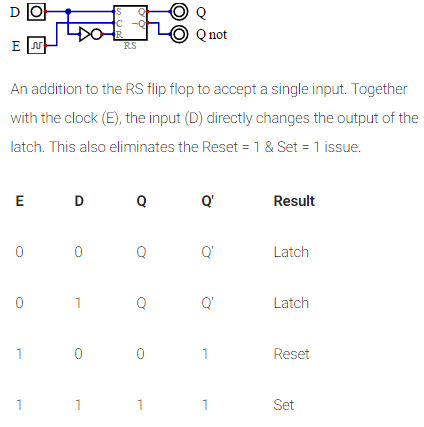
\includegraphics{dffl}
		\end{center}
		Used for registers/data.
	\end{figure}
	Chaining flip flops and their clock input stretches out inputs even more, how we use counters. 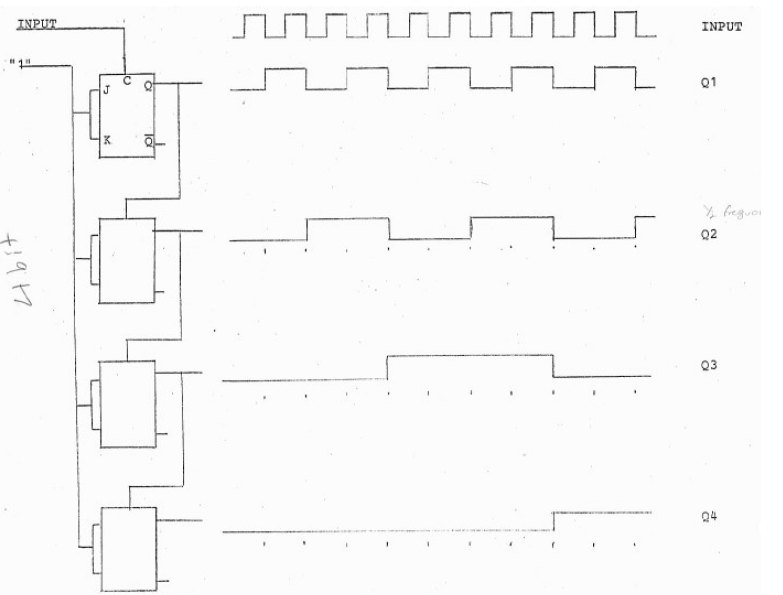
\includegraphics[scale=0.5]{bc}
	\subsection{Adders} How do we do grade school addition in binary at the hardware level? When adding 2 numbers together, we need a half adder for least significant bit (no carry) and full adders for all the other bits. Be careful of overflows and signed bits!
	\paragraph{Half-Adder} 2 bits in, sum \& carry out
		\begin{figure}[H]
			\caption{Half Adder, \href{https://www.allanwang.ca/notes/mcgill/comp273/0.php}{Allan Wang}}
			\begin{center}
				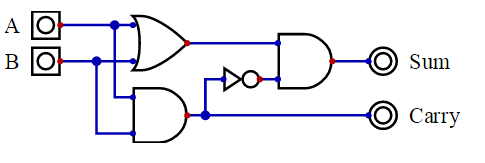
\includegraphics{ha}
			\end{center}
		\end{figure}
		If A \& B are both 1, then we will give 1 to carry and negate adding to sum.
	\paragraph{Full Adder} 3 bits in ($3^{rd}$ is carry), sum \& carry out
	\begin{figure}[H]
		\caption{Full Adder, \href{https://www.allanwang.ca/notes/mcgill/comp273/0.php}{Allan Wang}}
		\begin{center}
			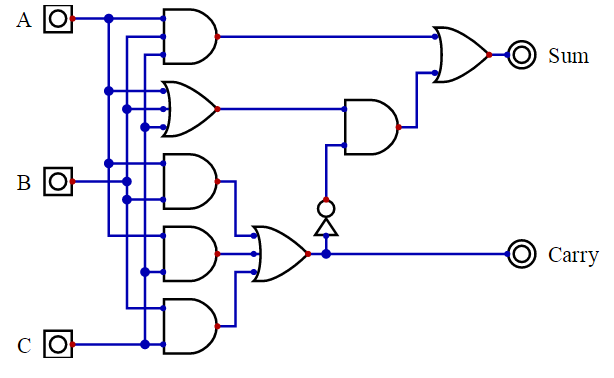
\includegraphics{fa}
		\end{center}
		Above is the more optimized version. Can just have 2 half adders and an or. Include simpler version with half-adders?
	\end{figure}
	\subsection{Combinatorial Networks} Premade circuits for specific purposes, readily available.
	\paragraph{Multiplexers} $2^a \to 1$ mux, $2^a$ inputs $x_0,\ldots,x_{n-1}$ and a single output z. Selector address a, with input signals $y_0,\ldots,y_{a-1}$, selects which $x_i$ to pass through z. Useful for when you have multiple signals but can only let one through at a time. Addressing, but with 1 output, z. \\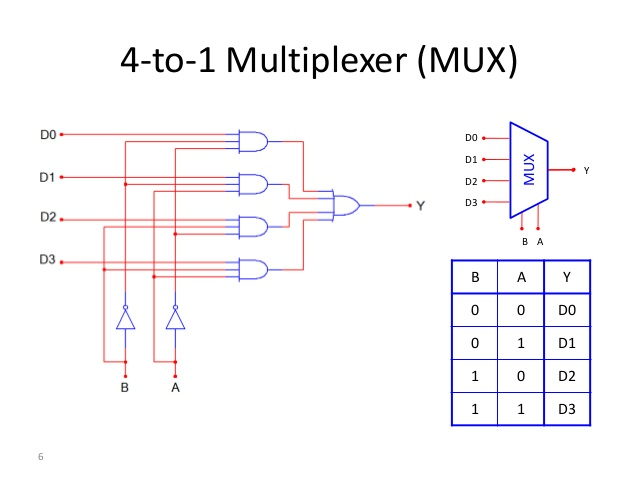
\includegraphics[scale=0.5]{multi}
	\paragraph{Decoders} $a \to 2^a$ decoder, gives out one of its $2^a$ outputs. Once again, like addressing, but selecting which you want to turn on. Like controlling switches. CPU sequencer is a decoder. 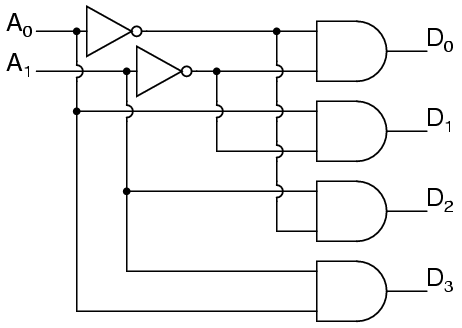
\includegraphics[scale=0.5]{decd}
	\paragraph{Encoders} Outputs a-bit binary number, $y_i$ equal to index of single 1 signal on among $2^a$ inputs $x_0,\ldots,x_{a-1}$. All of the xs are connected to an or gate, so if they're all off but $x_0$ is on, will show $0$.
	\paragraph{Programmable Combinatorial Parts} VIA Fuses that can be blown (disconnected) from enough current or VIA anti-fuses that are set(connected) from enough current. \\
	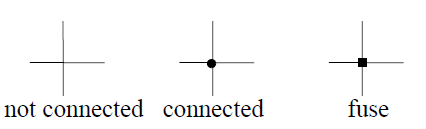
\includegraphics[scale=0.7]{fu}
	\subparagraph{PROM} Programmable read only memory, has anti-fuses that can be set, linked to decoder.
	\subparagraph{PAL} Programmable Array Logic, input wires are programmable, but output isn't.
	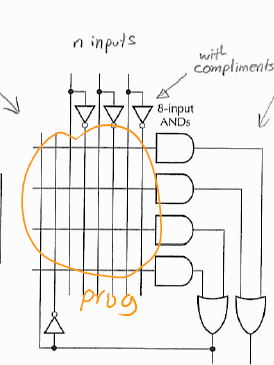
\includegraphics[scale=0.7]{pal}
	\subparagraph{PLA} Programmable Logic Array, input \& output programmable. 
	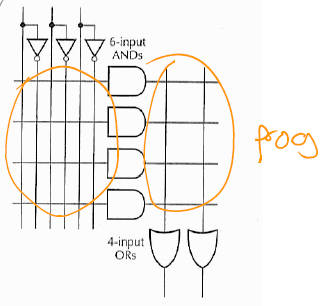
\includegraphics[scale=0.7]{pla}
	\section{In-Depth Classical CPU Analysis}
	\paragraph{Von Neumann Machine}
	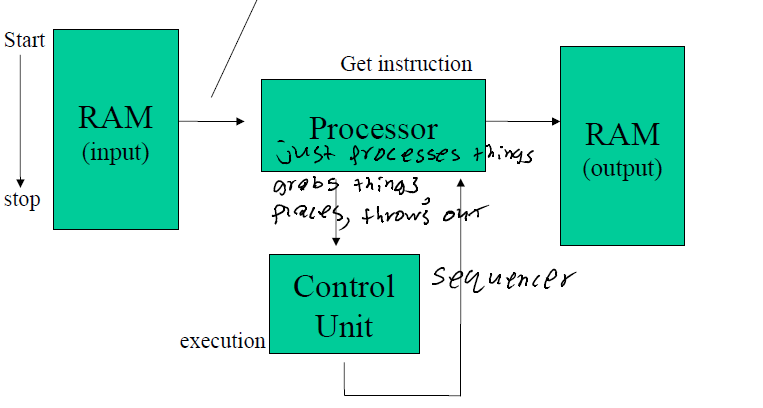
\includegraphics[scale=0.5]{vnm}
	\paragraph{Classical CPU Design}
	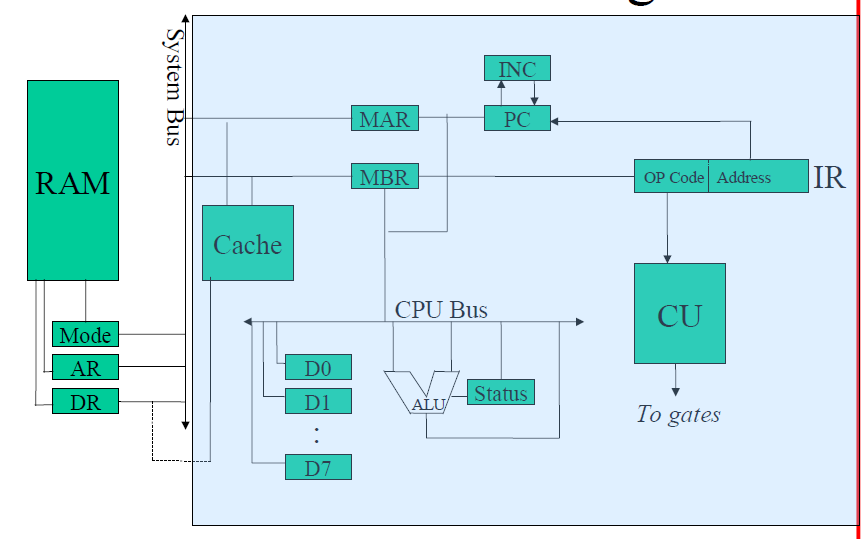
\includegraphics[scale=0.5]{ccpud} 
	PC = Program Counter or Instruction Pointer.
	\textbf{MAR}, memory address register, downloads instructions from PC, sends to AR. AR and MAR work a lot together, both address registers.
	\textbf{MBR}, memory buffer register, can contain many things (reason why it's called a buffer), like address, data from data registers. AR, DR and MAR, MBR work well together. INC is incrementer (override data in address), CU is control unit. Can add onto this diagram by adding peripherals on bus.
	\\ CPU does one instruction at a time in however x ticks it takes, then increments to next address to do next operation. Making things parallel \& local to avoid ticks and make it faster.
	\subsection{Instructions}
	Group of assembler instructions CPU supports. Standard size is usually the word size. Command that is formatted string of binary. Stored in RAM. Makes programs/algorithms.
	\paragraph{Program running (Classical CPU)}
	\begin{itemize}
		\item OS sleeps (no multithreading)
		\item 1. MAR $\gets$ PC
		\item PC $\gets$ PC+1
		\item 2. AR $\gets$ MAR
		\item DR $\gets$ RAM[AR]
		\item 3. MBR $\gets$ DR
		\item IR $\gets$ MBR
		\item CU $\gets$ IR(OP-CODE)
		\end{itemize}
	See instruction register for more info.
	\paragraph{Register vs RAM}
	Can give type to instructions, such that it goes through CPU registers or RAM. Through IR it does addition in 1 tick, but with RAM it has to go through several things, AR, MBR, IR in order to get what's at the RAM.
	\\ When program is done running, it tells the OS it can wake up now and stops program.
	\subsection{CPU Execution Cycle}
	\paragraph{Fetch}
	\begin{enumerate}
		\item PC $\to$ MAR, PC++
		\item MAR $\to$ RAM AR
		\item Read signal
		\item RAM DR $\to$ MBR $\to$ IR (or other register)
	\end{enumerate}
	\paragraph{Decode}
		\begin{enumerate}
			\item Do we need operands?
			\begin{enumerate}
				\item Get operands, using address in instruction to fetch each parameter, but last step goes to CPU register instead of IR and no incrementing of PC++
			\end{enumerate}
			\item OP-CODE $\to$ CU
		\end{enumerate}
		\paragraph{Execute}
		CU triggers gates to perform instruction
		\paragraph{Store}
		\begin{enumerate}
			\item Register with address $\to$ MAR
			\item Register with data $\to$ MBR
			\item Write signal sent to RAM AR and DR
		\end{enumerate}
		\subsection{Micro Instructions}
		Express operation of CPU, step by step. Syntax to follow.
		\\ CHANGE\_STATE $\gets $ OPERATION
		\begin{itemize}
			\item MACHINE(addr)
		\end{itemize}
		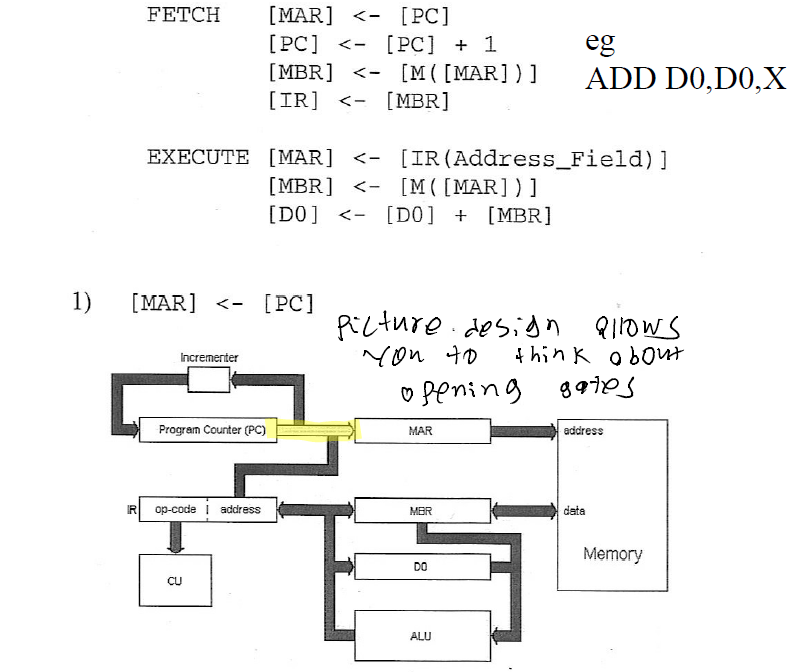
\includegraphics[scale=0.7]{mi1}
		\\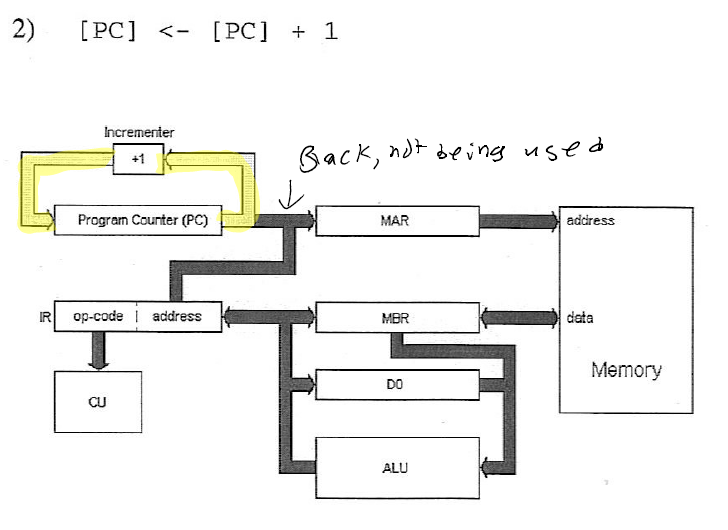
\includegraphics[scale=0.7]{mi2}
		\\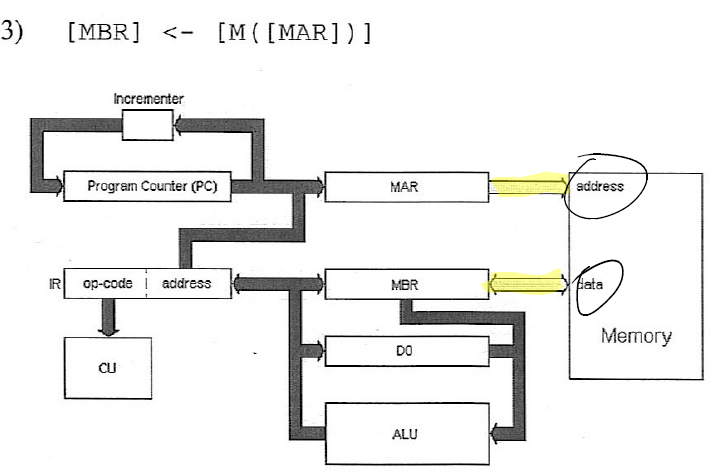
\includegraphics[scale=0.7]{mi3}
		\\ 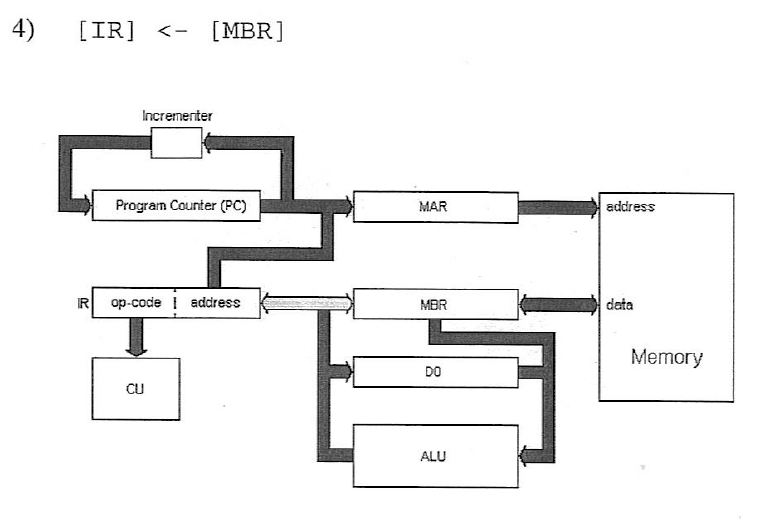
\includegraphics[scale=0.7]{mi4}
		\\ 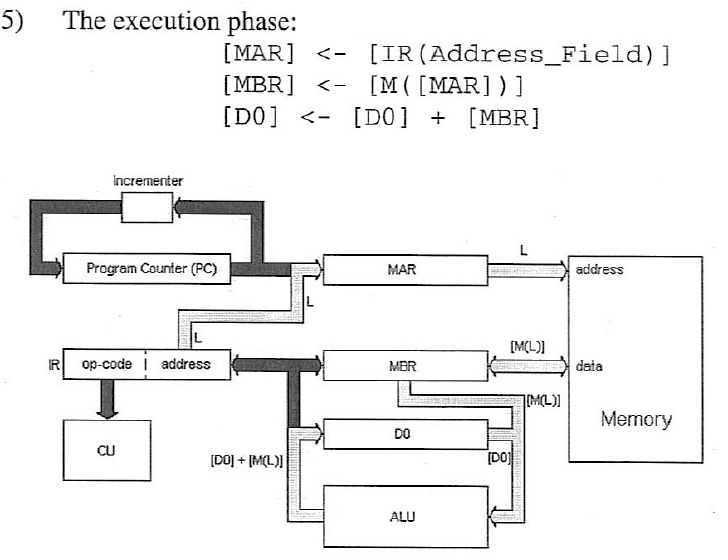
\includegraphics[scale=0.7]{mi5}
		\paragraph{Summary}
		~\\ 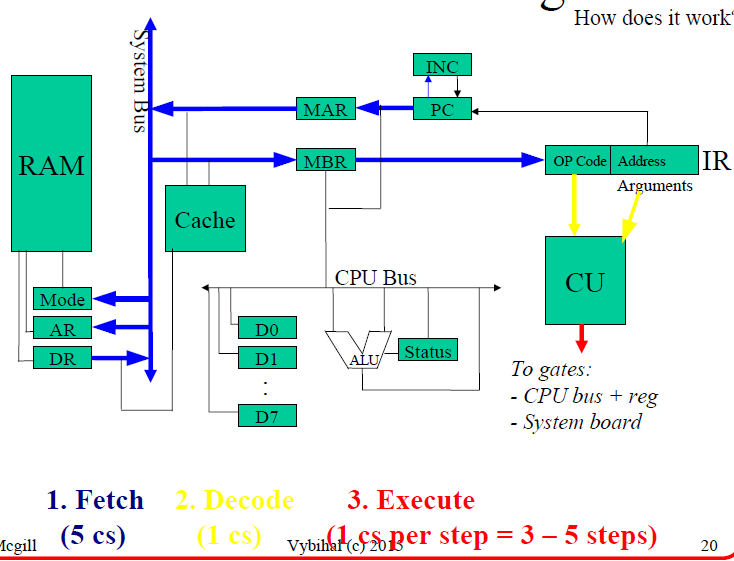
\includegraphics[scale=0.7]{ccpe}
	\section{Pipeline CPU Structure}
	When we look at the classical CPU architecture, we see that it is easy to build/cheaper and the bus allows flexibility of data movement. But, there are unused circuits and everyone has to share the same clock tick.
	\\ What about the pipeline CPU? The CPU \textbf{is} the bus. Only goes in one direction. Each instruction does a separate part at once, so you can have multiple instructions flowing through the pipeline at once (not executing simultaneously, more like doing different steps simultaneously). Pipeline instead of CPU loop.\\ \includegraphics[scale=0.7]{ppl}
	While fetching next instruction, can load current instruction. Can do 4 instructions at different phases at the ``same time". Need a lot of instruction registers, one at each stage (4). Two caches. Code/Load prediction has dumb(blind dump of code) vs smart(look ahead for goto/jump). The linearity/one way of the bus imposes restrictions on the language. All instructions go through the pipelin, need a wide 32 bit+ size bus.
	\paragraph{Effects on IR and CU}
	\begin{itemize}
		\item No longer 1:1 IR and PC
		\item Either one long CU or many small CUs
		\item 1 IR for every silo (data lock/gates), i.e. every step
		\\ \includegraphics[scale=0.8]{plir}
		\item Pipeline has to be gated
		\end{itemize}
		\paragraph{Fetch}
		\begin{itemize}
		\item Read address from PC, get instruction and send it out.
		\item Increment by 4 since 32-bit instructions.
\end{itemize}
		\includegraphics[scale=0.4]{fetch}
		\paragraph{Load \& ALU} 		\begin{itemize}
		\item Instruction goes to registers
		\item After op code and registers that are arguments, have $16$ bits leftover, have to sign extend, add $0$s in front
		\begin{itemize}
		\item This is for short constants, like offset of a LW instruction
		\item Some instructions don't require ALU, like $x=5$. Look at read data 2, skips ALU
\end{itemize}\includegraphics[scale=0.3]{load}

\end{itemize}
		\paragraph{Delayed Branching ALU}
		\begin{itemize}
		\item For things like BEQ, bottom ALU checks conditions like $X>Y$
		\item If true, will send op to upper ALU, new address with offset specified
		\item Will have to dump everything loaded after branch if we branch
\end{itemize}
		\includegraphics[scale=0.3]{dalu}
		\paragraph{Multi-Purpose ALU} ALU does different things depending on instruction, diff control codes. \\ \includegraphics[scale=0.4]{malu}
	\subsection{Summary Layouts}
	\begin{itemize}
	\item Can see that there are $4$ silos here
	\item Mux $\to$ multiplexer, decides which input to take in
\end{itemize}
	\includegraphics[scale=0.3]{slp}
	\begin{itemize}
	\item Bit Layouts
\end{itemize}
\includegraphics[scale=0.3]{slp2}
\begin{itemize}
\item 2 control units
\end{itemize}
\includegraphics[scale=0.2]{slp3}
\\ \includegraphics[scale=0.7]{psm}
	
	\section{Control Unit/Sequencer}
	CU is the portion of the CPU responsible for timing and triggering of data paths.
	\paragraph{Datapaths} Wires of CPU needed for particular tick/instruction.
	\paragraph{Instruction Format} Organization of bits in IR
	\paragraph{Micro-programming}
	\begin{itemize}
	\item Flat: one instr at a time
	\\ \includegraphics[scale=0.6]{fcu}
	\item Pipeline: Assembly execution of multiple
	\\ \includegraphics[scale=0.5]{pcu}
	\item Cores: Parallel exec
	\\ \includegraphics[scale=0.5]{ccu}
\end{itemize}
	\begin{itemize}
	\item Takes in an op-code register, associate numbers to instructions, like addressing. Open needed gates for specific instructions, mux
	\item The CU is like a decoder
	\item All commands belong to a certain family (see MIPS instructions)
	\item CU has a counter to tick the microinstructions of one instruction, op-code implemented via multiple sub-steps, works well if we make all instructions the same tick length
	\begin{itemize}
	\item When it overflows (gets to 0), resets itself for next instruction
\end{itemize}
	\item Pipeline has IR at each silo and 2 CUs, with 0-1 count
\end{itemize}
\paragraph{Buffers}
Multiple IR registers (buffers) for each instruction in pipeline.
	 \section{Performance}
	 \subsection{Hazards \& Faults}
	 \begin{itemize}
	 \item Hazard: danger to keep watch for
	 \begin{itemize}
	 \item Not being able to control what user can divide by, hazard
\end{itemize}
	 \item Fault: error has occurred
	 \begin{itemize}
	 \item Dividing by 0, fault
\end{itemize}
	 \item Stall: Normal CPU exec cycle lengthens
	 \begin{itemize}
	 \item Cache smaller than RAM
	 \item Small loops, try to fit it all in cache to run quickly
	 \item Otherwise it slows down to get parts in RAM
	 \item Stall might happen if CPU is running faster than code $\to$ stop pipelining and do classical or no-op
	 \item Instructions going from CPU to RAM, slower clock speed, stalls
\end{itemize}
	 \item Dump: Instructions after fault dumped from pipeline, re-loaded after fault handled
	 \item No-op: Extra instruction that doesn't do anything, between fault and next instruction, allows CPU to exec problematic instruction without many side-effects
\end{itemize}
hazard$\to$ fault $\to$ stall $\to$ dump or no-op
\\ ALU has a status register. If CU is in a certain operation (ex. div) and ALU gives an error, it'll stop program. Go back to PC or OS register, stop incrementor, OS looks at error.
\paragraph{Types of Hazards}
\begin{itemize}
\item Structural Hazards
\begin{itemize}
\item Bad combination of instructions, store/load in 1 Instructions
\item Illegal instruction or result
\end{itemize}
\item Control Hazards
\begin{itemize}
\item Branching (pipeline), making previous half executed instructions useless, comparison only happens at ALU
\end{itemize}
\includegraphics[scale=0.5]{bha}
\item Data Hazards
\begin{itemize}
\item Instruction depends on result of previous instruction, save only happens at 4th stage for pipeline
\begin{itemize}
\item Make CU check if instructions use same arguments
\end{itemize}
\item Use NOP or buffer to fix, can also reorder
\end{itemize}
\end{itemize}
\paragraph{Loss}
Calculate loss. At what stage did the fault happen? How many no-ops? How many things need to be reloaded after dump? How many instructions don't have faults (full speed)?
\\ The performance loss experienced $\to E[Loss]=p(Loss)*cost$, stalls happen $17\%$ of the time, still worth it to use pipeline.
\paragraph{Solutions}
\begin{itemize}
\item Insert no-ops or reorder instructions (reordering branch or instructions that conflict)
\item Assume branch will always fail (bad, not used)
\item Assume branch success based on type
\begin{itemize}
\item Function calls good
\item Backwards jumps, probably loops, good
\item If statements, no
\end{itemize}
\end{itemize}
\subsection{Performance Issues}
\begin{itemize}
\item Clock ticks: Number of clock ticks required to perform activity, only reliable measure
\item Cycles: count of number of micro instructions to perform an activity
\item CPU execution time = $n$ instructions in prog $\times$ $Y$ ticks per instr $\times$ $Z$ seconds per tick
\begin{itemize}
\item Classical CPU, different ticks for different instructions
\item Pipeline, all the same
\end{itemize}
\end{itemize}
\subsection{CPU Exception Handling}
Why?
\begin{itemize}
\item Bad machine language Binary
\item Bad arithmetic
\item Incorrect address
\end{itemize}
Supporting registers:
\begin{itemize}
\item Expection Program Counter register (EPC), stores addr of bad instr
\item Cause, has error code
\item Jump to reserved cache mem for exception assembler code
\end{itemize}
Assembler implementations
\begin{itemize}
\item Jump to OS exception handler
\item Jump to code in user program to handle it
\end{itemize}
What ends up happening: Exception handling hardware built into CPU, has default PC address locations (hardwired) to interrupt. Error happens, PC stored into EPC, PC gets default address relating to type of error. OS or programmer has code at that address to handle.
\section{CPU \& Chipsets}
\subsection{CPU}
What does the CPU system consist of?
\begin{itemize}
\item General purpose registers
\item ALU
\item Cache
\item OS registers
\item System-Board registers
\item Supporting chipsets
\end{itemize}
\paragraph{Supporting CPU Registers}
Running 2 programs on a computer, shouldn't interfere with each other.
\begin{itemize}
\item Process Boundary Register: has upper bound and lower bound for jump/branch statements compare PC with illegal situations. Protect processes, OS and zero page. OS' job to load registers.
\\ \includegraphics[scale=0.7]{pbd}
\end{itemize}
Some don't have upper and lower boundary registers, have OS boundary register instead, prevents processes from addressing into OS space, programs can damage each other, but not OS. For special instructions, we can use assembler instructions (like syscall).
\subsection{Chipsets}
Chips \& circuitry to support CPU, your CPU needs a team.
\begin{itemize}
\item On Die chip sets: circuitry on CPU die, same Board
\item On Board chip sets: circuitry on system board, usually clos to CPU, different bus
\end{itemize}
\paragraph{Some chipsets}
\begin{itemize}
\item Co-processors
\begin{itemize}
\item Math, matrix, graphics GPUs
\item MIPS only has an integer ALU, has a co-processor to do floating point arithmetic
\end{itemize}
\item ROMS
\begin{itemize}
\item Support for video, basic graphics
\item ASCII
\item Ports to commmunicate, peripherals
\end{itemize}
\end{itemize}
\subsection{Co-Processors}
Like CPU, but CPU has everything, co-processor only has the things it needs to do what it was made for, i.e. math. Floating point numbers are stored very differently from integers, need a co-processor to do arithmetic.
\\ \includegraphics[scale=0.7]{fpa}
\paragraph{Grade School Multiplication}
Works the same way as decimal multiplication:
\begin{enumerate}
\item Right most digit of multiplier multiplies multiplicand
\item Write answer below digit
\item Next digit of multiplier, go to step 1 (writing underneath next digit implies shifting)
\item Sum
\end{enumerate}
Really just need to AND everything, $1\times 1=1, 0\times 1=0$. Floating point numbers are 32 bits, will take 32 ticks per floating multiplication, convert to integer when possible as this is a huge stall.
\paragraph{Integer Multiplier Circuit} Note that we have 3 $64$ bit registers here!\\
\includegraphics[scale=0.7]{imc}
\paragraph{Improvement I} Change multiplcand \& multiplier to $32$, right shift product register instead, Will constantly have a line splitting the $64$ bit product register, because right most bits are only added a few times, least significant is not added, 2nd least is added once, etc. \includegraphics[scale=0.8]{aon}\\
\includegraphics[scale=0.3]{imci}
\paragraph{Improvement II} No more multiplier register, placed in answer part of product instead.\\
\includegraphics[scale=0.3]{imcii}
\\ To do negative multiplication, convert to a positive value and check signs at the end
\\ Multiplication by $2^i$ does not require multiplication (much faster), just shift left $i$ times
\paragraph{Integer Division} Same as grade school division\\
\includegraphics[scale=0.2]{dvf}
\\~ \includegraphics[scale=0.4]{dva}
\\~ \includegraphics[scale=0.7]{idc}
\paragraph{Optimization}
\begin{itemize}
\item  Shift remainder left instead of divisor right, make divisor reg 32 bits
\item Remove quotient register, put in right half of remainder
\item $1$ cannot be first bit in quotient, shift remainder left by $1$ to do one less iteration
\end{itemize}
\includegraphics[scale=0.6]{dvi}
\\ \includegraphics[scale=0.3]{dvix}
\subsection{Multiprocessing}
\paragraph{Types of computers}
\begin{itemize}
\item Single CPU, one CPU chip, any type (flat, pipeline, hyper threaded)
\\ \includegraphics[scale=0.7]{sc}
\item Multi-CPU, more than one CPU chip, any type
\\ \includegraphics[scale=0.7]{mcc}
\item Single Core, like single CPU chip, but optimized. Has a bridge (connected to buses) to connect core with rest of system board
\\ \includegraphics{scc}
\item Multi-Core, single cpu chip with multiple processors, aka Chip Multi-Processor (CMP). Bus interface shared (unlike Multi-CPU), to have same data
\\ Cache instructions, like a pipeline, but faults more likely
\\ \includegraphics[scale=0.7]{mccc}
\paragraph{Programs}
\begin{itemize}
\item Program is a compiled algorithm stored on disk, static
\item Process is executing version of program in RAM, static \& dynamic
\item Thread are instructions currently being run
\begin{itemize}
\item Process can have many threads
\item Thread is an instance of process
\end{itemize}
\end{itemize}
\end{itemize}
For multi-core, threads run in parallel, once for each core. Can have hyperthreading and have queues in each core. Fork a program to split across multiple cores. The more cores, the more the advantages get smaller since they all need to communicate with each other. Multicore because we can't make things go faster than speed of light, so we need more of them.
\paragraph{OS Core Management}
OS treats each core as a unique processor. OS schedules processes and threads to diff cores
\begin{itemize}
\item Special purpose core assignment: OS reserves cores for types of apps
\item Dedicated application assignment: Application attached to core, always done on that core. Shareable with other processes
\item Core pooled assignment: Queue manages all proceses, process at front gets any available core
\item Simple Management
\begin{itemize}
\item Queue of processes to execute
\item Each core assigned to waiting process
\item After n microsec, release core and loop
\end{itemize}
\item Complex Management
\begin{itemize}
\item One process has multiple threads in queue
\item Need to share data, put on a core that can share
\item Hardware for data access conflicts
\end{itemize}
\end{itemize}
\paragraph{Problem}
\begin{itemize}
\item Uniqueness of threads
\begin{itemize}
\item 1 thread per program? Programs all execute at the same time
\item N threads per program? (like a browser with multiple windows)
\begin{itemize}
\item They have to coordinate with each other, overhead to manage
\item $N>6$, overhead starts to be more than speed improvement
\end{itemize}
\end{itemize}
\end{itemize}
\paragraph{Parallelism}
\begin{itemize}
\item Single core, instruction level parallelism $\to$ pipeline
\item Thread-level parallelism (TLP), multi-core
\begin{itemize}
\item Each core gets a part of program to execute
\item Single cores cannot take advantage of TLP, future will involve multi-cores exploiting TLP
\end{itemize}
\includegraphics[scale=0.7]{mct}
\end{itemize}
\paragraph{Single Instruction Multiple Data (SIMD)}
\begin{itemize}
\item Ex. Modern GPU
\item Matrix of data
\item 1 instruction executed on all cells at same time
\item One cell is a core
\end{itemize}
\paragraph{Multiple Instruction Multiple Data (MIMD)}
\begin{itemize}
\item Multi pipeline CPU
\item 1 pipeline per core
\item Shared RAM
\item Each core has own caches
\item Core itself is SIMD
\item Chip as a whole is MIMD
\end{itemize}
\paragraph{Simulataneous multi-threading (SMT)}
\begin{itemize}
\item Multiple independent threads executing at same time on same core
\item Can do integer operation on one thread and floating point on another (2 ALUs)
\item Not really parallel, $30\%$ threading, virtual processor, does not have resources for each core like Multi-core
\item Can have multi-cores with SMT
\item Intel calls SMT hyper-threads
\end{itemize}
\paragraph{Memory Types}
\begin{itemize}
\item Shared memory, shared between all processors
\item Distributed memory, each processor has own memory
\item Lots of computers have both
\includegraphics[scale=0.3]{mts}
\end{itemize}
\paragraph{Private vs Shared Cache}
\begin{itemize}
\item Private is closer to core, faster access, less contention
\item Shared, different cores can access the same thing, more space for big stuff
\end{itemize}
\paragraph{Problems}
\begin{itemize}
\item  Contention: More than one core needs access to same cache, one has to wait, need circuitry to handle
\item Cache coherence: Private caches, need data to be consistent, each core should perceive memory as shared
\begin{itemize}
\item Core 1 changes a value, core 2 reads the old value
\item Solution: Inter-core bus, looks at MAR, addresses being used, issues faults (invalidation + snooping)
\begin{itemize}
\item Core writes to cache, then all other copies $\to$ invalid
\item All cores snoop the bus connecting cores for write ops
\end{itemize}
\end{itemize}
\end{itemize}

\paragraph{Memory Hierarchy}
\begin{itemize}
\item Not shared: Pipeline, L1 private
\item Shared: L2 (sometimes private), L3, RAM
\item Special: SMT, all caches shared
\end{itemize}
	\section{MIPS}
	\subsection{Instructions}
	4 instruction classes:
	\\ \includegraphics[scale=0.7]{4ins}
	\paragraph{Effects on CU}
	~\\\includegraphics[scale=0.2]{cuo}
	\\ Different pathways for different types of instructions.
	\paragraph{R-Type Fetch}
	~\\ \includegraphics[scale=0.7]{rty}
	\paragraph{R-Type Load}~\\ \includegraphics[scale=0.7]{rtl}
	\paragraph{R-Type ALU}~\\ \includegraphics[scale=0.7]{ralu}
	\paragraph{R-Type Store}~\\ \includegraphics[scale=0.7]{rstr}
	\subsection{Assembler Code}
	\paragraph{Scope} All peripherals and system components accessible by instructions. Can access hardware through RAM (zero page), but you need to know address, binary format, command, status \& data registers. Access to hardware requires privileged instructions.
	\begin{itemize}
	\item Privileged mode allows all registers protecting OS to be accessible (like boundary registers)
	\item Non-privileged is the opposite, used in this class
\end{itemize}
\paragraph{Compiling High Level Languages} Code $\to$ Compiler$\to$ Assembler $\to$ linker (with library and loader) $\to$ executable
\begin{itemize}
\item Compiler checks syntax, coverts to assembly
\item Assembler checks for syntax, converts to machine code
\item Linker verifies library calls exist, merges library into program, adds special OS functions , determines memory locations that code will occupy, resolves references, ensures no undefined labels
\item Loader \& Loading
\begin{itemize}
\item Loading: Puts program into RAM, notifies OS
\item OS responsible to pass CPU to program later
\item Loader: subroutine, knows how to put program into RAM and notify OS
\begin{itemize}
\item Three types of OS
\item Loader function to be inserted as first instruction of program, done by linker
\item Built-in function, require program to call it
\item Require data record for parameters and do the whole process internally, no loader
\end{itemize}
\end{itemize}
\end{itemize}
We need the outputs and versions to match each other for the program to execute/work.
\\ Assembly program consists of the above, without a compiler, going directly from source code to assembler
\paragraph{Assembler} Converts assembler text file into .o file, has instructions and directives
\paragraph{Directives}
\begin{itemize}
		\item Comments indicated by \#
		\item .text indicates code is after this
		\item .globl name of LABEL $\to$ where is main program
		%\item syscall calls system to temporarily wake up to do something, like print
		\item .data indicates things stored and whatnot
		\item LABELS: define label's location, LABEL references its location
		\end{itemize}
\paragraph{Two-Pass Assembly}
Building to linker:
\begin{itemize}
\item Pass 1: builds symbol table, indentifies labels, determines offset addresses of identifiers
\begin{itemize}
\item Scans source, top to bottom
\item Count number of bytes in instructions passed to see how many bytes long the program is
\item Find a label, add to symbol table with offset from beginning of program
\item First instruction/label receives a base address in the symbol table, all others are just offsets from that address
\\
\begin{tabular}{|c|c|}
LABEL&OFFSET
\\ \hline main & x
\\ int a & +3 (offset from x)
\end{tabular}

\end{itemize}
\item Pass 2: builds machine language program, 1-to-1 map
\begin{itemize}
\item Scan source, top to bot again
\item One line of assembly is one line of machine, convert op-code \& args
\item Assembly Template, just like Symbol Table, but has addresses (with offsets) and instructions in binary
\end{itemize}
\end{itemize}
\paragraph{Unix Loading Algorithm}
\begin{itemize}
\item Read file header, determine CODE and DATA size req
\item Find space in RAM for prog, set BASE addr
\item Copy instructions and data into RAM
\item Copy args onto run-time stack
\item Assign SP to next free stack position, IP to first instr
\item Clear registers
\end{itemize}
\section{Examples}
	\paragraph{An example of Copying from RAM to a Slot}
	\includegraphics[scale=0.5]{rmstr.png}
	In this example, we'd like to copy 10 letters from RAM to an arbitrary slot on a traditional system board. We must loop through as follows:
	\begin{enumerate}
		\item Open gate 0 \& 1, close all other gates.
		\item Wait for tick.
		\item 1 character passes.
		\item Go back to step 2.
		\item Once all 10 characters are written, ``supervisor" (later, central unit?) closes all gates and the operation is done.
		\end{enumerate}
		\paragraph{Can a single byte in RAM and a single CPU instruction in RAM both exit RAM at once?}
		~\\ No, not possible with traditional system board. You can do each one very quickly, but not simultaneously.
		\paragraph{What does the circuit of a full 2-byte r/w memory look like?}
		Size of RAM is 2-byte, need 16 flip flops. Need a r/w register, data register and some sort of addressing system (many gates, only opening access to 1 bit at a time). Clock controls it all.
		\paragraph{ALU Questions}
		\subparagraph{What do we need to assume about our data to build an ALU}
		Size of inputs \& outputs.
		\subparagraph{How would the assumptions impact the design of the ALU?} Limit capacity to do arithmetic, depending on size of data.
		\subparagraph{4-bit integer ALU with addition and subtraction?} 2 Half-adders.
		\subparagraph{Upgrading size?} Add more half adders, bigger output.
		\paragraph{Binary Code Decimal}
		7 segments (calculator LED), depending on which bits are on, display that number. Uses addressing.
		\paragraph{Given 2 bit binary number, use PLA to send out single bit value for each binary value.} (Like a decoder) \\
		\includegraphics[scale=0.8]{pladd}
		\paragraph{Temperature stored in a register as a binary number, set off alarm when temp is $\geq$ 500} Do all the situations 5+, then put them all into an or.
		\paragraph{$2$ GHz computer}
		CPU that executes 1 instruction/20 ticks
		\\ How long to run linear program of 1000 lines of code?
		\\$T=1000\times 20/2\times10^9=0.00001$ sec
		\paragraph{Comparing Pipeline \& Classical}
		Given ratio of program instructions (how much \% is loads, stores, etc.) and how long each step takes. Use: $time=instructions \times ticks/instr \times secs/ticks$
		\includegraphics[scale=0.6]{vfx}
		\section{Exercises}
		\subsection{Circuits}
		\begin{itemize}
			\item Make a circuit with a truth table
			\item Simple 3 bit increment with 1 circuit, no adder
			\item 2's complement circuit
			\item Circuit picking 1 bit out of 2 bits, given a 1 bit number
			\end{itemize}
	% \section{Readings}
	% \paragraph{Computer Organization \& Design Textbook}
	% Readings correspond to the \textbf{$4^{th}$} edition of the textbook, not the $5^{th}$.
	% \begin{itemize}
	% 	\item Chapter 1
	% 	\item Chapter 2.4
	% 	\item Appendix C1 to C11
	% 	\item Chapter 4
	% 	\item Appendix D
	% \end{itemize}
\end{document}
%%% Local Variables:
%%% mode: latex
%%% TeX-master: t
%%% End:
